\section{Zobrazovací prvky}
-popis technologií LCD, OLED, plazma, elektronický inkoust, QLED. Základní struktury, popis funkce a srovnání výhod a nevýhod jednotlivých technologií.

\subsection{LCD}
Barevné nebo monochromatické pixely jsou umístěny před zdrojem
světla.\\
Každý pixel je rozdělený do tří subpixelů, a to červeného, zeleného a
modrého (tedy RGB). Svítivost každého pixelu je možné kontrolovat
nezávisle na ostatních, jejich kombinací lze pak
dosáhnout milionů barev.\\
Každý pixel LCD se skládá z molekul tekutých krystalů uložených mezi
dvěma průhlednými elektrodami a mezi dvěma polarizačními filtry,
přičemž osy polarizace jsou na sebe kolmé.\\
Molekuly tekutých krystalů jsou bez vnějšího elektrického pole ovlivněny
mikroskopickými drážkami na elektrodách. Drážky na elektrodách jsou
vzájemně kolmé, takže molekuly jsou srovnány do spirálové struktury a
stáčí polarizaci procházejícího světla o 90 stupňů, což mu umožňuje projít i
druhým filtrem.\\
Polovina světla je absorbována prvním polarizačním filtrem, kromě toho je
ale celá sestava průhledná.\\
\textbf{Princip:} https://www.youtube.com/watch?v=rR0YbNjDoVU
\subsubsection{LCD rozdělení}
\textbf{Pasivní STN (Supertwist Nematic):}\\
Jednodušší ‐ tvoří ji dva substráty skla, jeden tvoří sloupce a druhý řady.
Elektrický náboj přivádíme k určitému bodu v určité řadě a sloupci.\\
\textbf{Aktivní TFT (Thin‐Film Transistors):}\\
Je tvořena tenkovrstvými tranzistory . Pomocí této metody lze přesně ovládat
velikost napětí na krystalech a tím i ovládat jas displeje.\\

\subsection{OLED}
OLED (Organic Light Emitting Diodes)\\
Přímo generují světlo\\
Účinnost běžně 18‐22 lm/W\\
pro bílé OLED až 50 lm/W)\\

\subsubsection{Základní vlastnosti}
Plně barevné displeje s přímou barevnou emisí\\
Vysoký kontrast\\
Velmi tenký (cca 1mm) a velmi lehký\\
Možnost použití flexibilního pružného substrátu => ohebný displej\\
V celku jednoduchá struktura => nízké výrobní náklady a tedy i cena\\
Nízká spotřeba ne více než 30‐60 mW\\

\subsubsection{Princip}
Pracují na principu elektroluminiscence\\
Klíčový je organický materiál obsahující molekulární strukturu, známou
jako luminofor (provádí emisi světla)\\
Emise světla – rekombinací excitovaných párů elektron – díra, nadbytek
energie je vyzářen v podobě fotonu, tj. světelného záblesku\\
Jako polymerní luminofory se tedy používají různé deriváty materiálu
PPV, obvykle poly(p‐phenylene vinylene) a poly(fluorene)\\

\textbf{Anoda (první elektroda):}\\
tvořená z oxidu india dotovaného oxidem cínu (ITO) (transparentní keramický materiál za normálního stavu vodivý).\\
\textbf{Katoda (druhá elektroda):}\\
je obvykle vyrobena z kovu ‐ nejčastěji hliníku.\\

    \begin{figure}[h]
   \begin{center}
     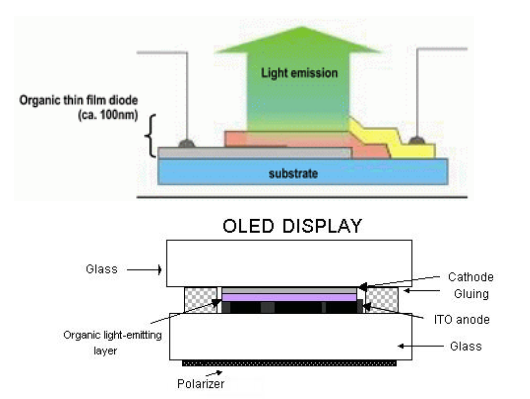
\includegraphics[scale=0.4]{images/OLED.png}
   \end{center}
   \caption{Princip OLED}
  \end{figure}
\subsubsection{Výhody}
Snadno zhotovitelné ‐ v principu může potřebné prvky vytvořit na
folii příslušným způsobem vybavená inkoustová tiskárna\\
větší úhel pohledu\\
velmi rychlý reakční čas, menší než 1 $\mu$s\\
hodnoty úrovně černé a kontrast jsou minimálně stejně dobré\\
nepotřebuje nasvícení pozadí ‐ umožňuje výrobu extrémně tenkých displejů\\
Možnost jednoduchého provedení flexibilních (ohebných) displejů\\
Displeje s úhlopříčkou nad 40"\\

\subsubsection{PMOLED}
PMOLED ‐ pasivní OLED displej\\
Nejjednodušší varianta\\
Základ tvoří mřížková matrice vzájemně překřížených vodičů. V místě křížení se vodiče připojeny k elektrodám (katodám, resp. anodám) OLED struktury a vznikají tak jednotlivé pixely.\\
K emisi světla dojde impulsem na příslušeném řádkovém a sloupcovém vodiči\\
Čím je větší proud impulsu, tím jasněji pixel září\\
\subsubsection{AMOLED}
AMOLED (Active‐matrix OLED) aktivní struktura OLED displeje\\
Každý pixel řízen vlastním tranzistorem (přesně řídí proud do struktury OLED) a lze tak regulovat jas\\
Vyznačují vyšší zobrazovací frekvencí\\
Ostřejším vykreslením obrazu\\
Nižší spotřebou\\
Pod každým pixelem je struktura dvou tranzistorů s kondenzátorem, kde jeden
tranzistor řídí proud pro nabíjení a vybíjení kondenzátoru, zatímco druhý slouží jako
napěťový stabilizátor, pro zajištění konstantní velikosti proudu.\\
\textbf{Nevýhody:} výrazně složitější struktura displeje a tedy i vyšší
cena.\\
\pagebreak
\subsection{Plazma}
    \begin{figure}[h]
   \begin{center}
     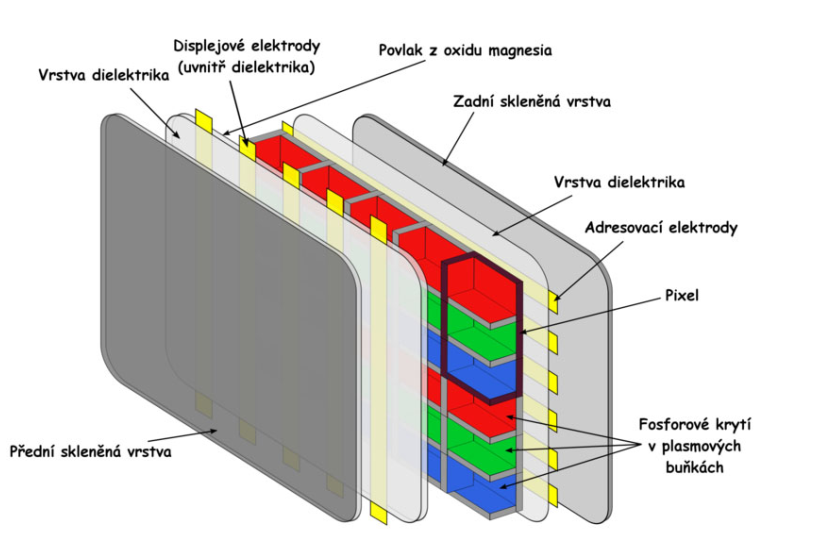
\includegraphics[scale=0.4]{images/Plazma.png}
   \end{center}
   \caption{Plazmová obrazovka}
  \end{figure}

Střídavé napětí,\\
napětí je udržováno těsně pod ionizační hladinou,\\
Neon a Xeon jsou excitovány při návratu do své orbitální hladiny se uvolňuje ultrafialové záření, které způsobí excitaci atomů luminoforu => uvolnění viditelného záření.\\
Intenzita každého subpixelu je určována počtem a šířkou napěťových pulsů, které dostává
buňka během každého snímku.
Standardní metoda určuje 256 úrovní nabití pro každý subpixel, protože každý snímek je
rozdělen na 8 podsnímků ovládaných 8bitovým slovem. Celá tato technologie se nazývá ADS
(Address/Display Separated)\\
\textbf{Výhody:}\\
Vynikající kontrastní poměr\\
Vynikající pozorovací úhly kolem 160–170$^{\circ}$\\
Jas až 1000 lx\\

\textbf{Nevýhody:}\\
V tmavých scénách se barvy blízké černé slévají v jednu a přechody nejsou zdaleka plynulé\\
rozteč bodů okolo 0,3 mm\\
vyšší spotřeba\\
tloušťka 6 cm\\
\subsection{E-ink}
Rozlišení jen 167 ppi (600x800)\\
16 stupňů šedé\\
Rychlost 0,5 s\\
Pro udržení obrazu není potřeba energie\\
\subsubsection{Princip}
E-INK je složen z miliónů miniaturních mikrokapslí (Microcapsules) ) o průměru cca lidského vlasu. Každá obsahuje pozitivně nabité bílé částice a negativně nabité částice černé, které "plavou" v opticky průhledné tekutině (Clear fluid). Ty právě tvoří černou nebo bílou plochu určující barvu daného pixelu. Ta se ovládá pomocí elektrického pole mezi elektrodami (transparent electrodes), podobně jako klasické LCD. Dá se tedy k řízení využít TFT spínací matice, kde každý pixel je ovládán separátním tranzistorem.
    \begin{figure}[h]
   \begin{center}
     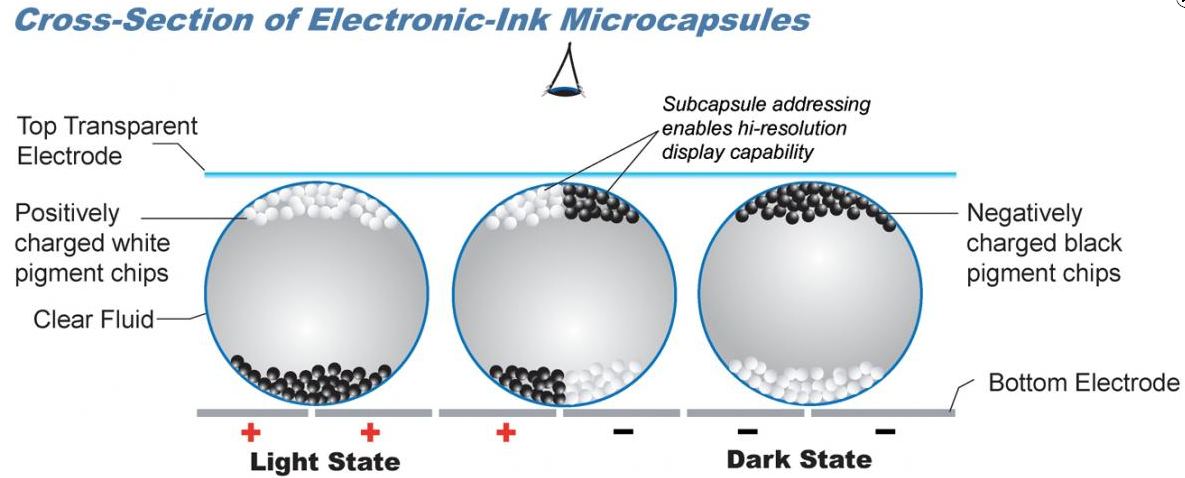
\includegraphics[scale=0.4]{images/EINK.png}
   \end{center}
   \caption{Princip E-ink}
  \end{figure}

\textbf{Výhody:}\\
Fantastická čitelnost displeje při zobrazení textu\\
Nízká spotřeba (energie se z článku odebírá pouze při překreslování, ve
statickém režimu je spotřeba nulová)\\
\textbf{Nevýhody:}\\
Velká citlivost na ohyb\\
Malé rozlišení\\
Nutné okolní osvětlení\\

\subsection{QLED}
Displej s kvantovými tečkami je zobrazovací zařízení využívající kvantové tečky (QD), polovodičové nanokrystaly, které mohou produkovat čisté monochromatické červené, zelené a modré světlo.

Fotoemisní částice kvantových teček se používají v podsvícení LCD a/nebo v barevných filtrech displeje. Kvantové tečky jsou excitovány modrým světlem ze zobrazovacího panelu a vyzařují čisté základní barvy, což snižuje světelné ztráty a barevné přeslechy v barevných filtrech, zlepšuje jas displeje a barevný gamut (Gamut, resp. barevný gamut, je dosažitelná oblast barev v určitém barevném prostoru). 

Světlo prochází vrstvou QD filmu a tradičními RGB filtry vyrobenými z barevných pigmentů nebo QD filtry s převodníky červené/zelené barvy QD a modrým průchodem. Ačkoli se technologie barevných filtrů QD používá především v LCD displejích s podsvícením LED, je použitelná i v jiných zobrazovacích technologiích, které používají barevné filtry, jako jsou modré/UV AMOLED/QNED/MicroLED zobrazovací panely
\subsubsection{Princip}
Kvantové tečky jsou buď fotoemisivní (fotoluminiscenční), nebo elektroemisivní (elektroluminiscenční), což umožňuje jejich snadné začlenění do nových architektur emisních displejů. Kvantové tečky přirozeně produkují monochromatické světlo, takže při barevné filtraci jsou účinnější než zdroje bílého světla a umožňují sytější barvy, které dosahují téměř 100 \% barevného gamutu
    \begin{figure}[h]
   \begin{center}
     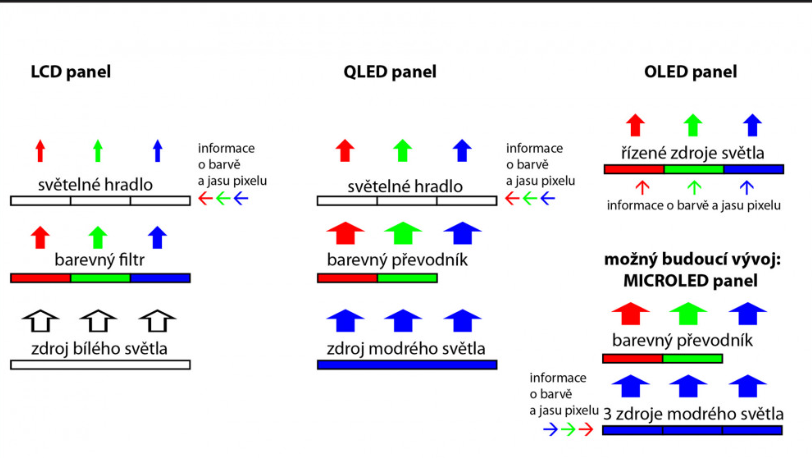
\includegraphics[scale=0.6]{images/QLED.png}
   \end{center}
   \caption{Porovnání LCD, QLED a OLED}
  \end{figure}















